\documentclass[tikz,border=10pt]{standalone}
\usepackage{tikz}
\usetikzlibrary{calc}
\begin{document}
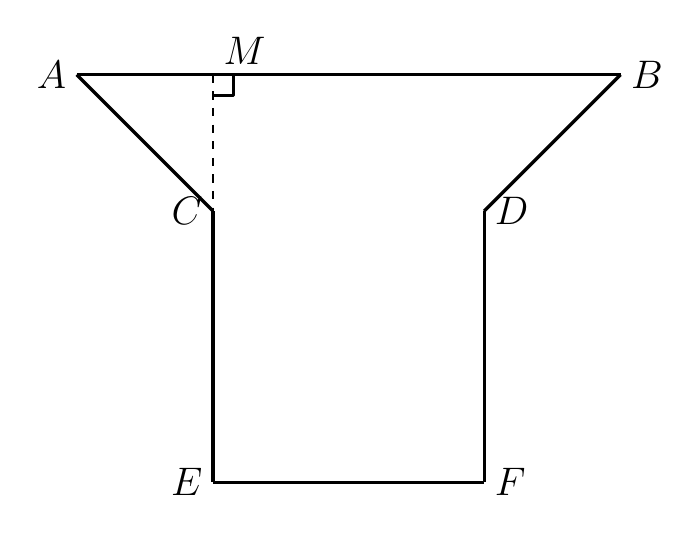
\begin{tikzpicture}[line join=round, line width=1.0pt, font=\fontsize{14.5}{17.4}\selectfont]
  % Coordinates: scale s = 0.018223 cm/px, origin at ink-bbox centre (256.5, 194.5) px
  \coordinate (A) at (-3.4532, 2.3599);
  \coordinate (B) at (3.4532, 2.3599);
  \coordinate (M) at (-1.7221, 2.3599);
  \coordinate (C) at (-1.7221, 0.6287);
  \coordinate (D) at (1.7221, 0.6287);
  \coordinate (E) at (-1.7221, -2.8154);
  \coordinate (F) at (1.7221, -2.8154);

  % Solid outline (thick)
  \draw[line width=1.2pt] (A) -- (B);   % top edge AB
  \draw[line width=1.2pt] (D) -- (F);   % right vertical DF
  \draw[line width=1.2pt] (E) -- (F);   % bottom edge EF
  \draw[line width=1.2pt] (A) -- (C);   % diagonal AC
  \draw[line width=1.2pt] (B) -- (D);   % diagonal BD
  \draw[line width=1.2pt] (C) -- (E);   % lower stem C-E, solid

  % Dashed vertical from M down to C only (no overhang above M)
  \draw[dashed] (M) -- (C);

  % Right-angle mark at M (arms right and down, side 0.26 cm)
  \draw (-1.4624, 2.3599) -- (-1.4624, 2.1002) -- (-1.7221, 2.1002);

  % Labels
  \node[above right] at (M) {$M$};
  \node[left] at (A) {$A$};
  \node[right] at (B) {$B$};
  \node[left] at (C) {$C$};
  \node[right] at (D) {$D$};
  \node[left] at (E) {$E$};
  \node[right] at (F) {$F$};
\end{tikzpicture}
\end{document}